\chapter{\textit{Modelagem dinâmica}}


\section{Modelagem do quadrirrotor}
Um quadricóptero é um tipo de veículo aéreo não tripulado(VANT), caracterizado por ter quatro rotores, que podem ser dispostos em diversas configurações. O Parrot Mambo, utilizadop nesse trabalho dispõe de uma configração em X, sendo que cada rotor pode variar sua velocidade de direção de giro de maneira independente.
Para se estudar as características dinâmicas e o sistema de controle do quadrirrotor deste trabalho é necessário entender como as forças que interagem com o corpo se relacionam. A análise dinâmica de um drone pode ser dividida na dinâmica de corpo rígido, dinâmica translacional, na cinemática e dinâmica de atitude, nas forças agindo sobre o corpo e o controle. Assim, neste capítulo será apresentado essa análise.

\subsection{Sistemas de coordenadas}

Para modelagem dinâmica de um quadricóptero pode-se começar considerando-o como um corpo rígido e aplicando as leis de Newton, que necessitam de um referencial inercial (que não está acelerando nem rotacionando) para serem válidas, bem como definir um sistema de coordenadas local que se desloca e rotaciona com o quadricóptero.
Nesse estudo, por conveniência escolhemos como sistema de coordenadas inercial o sistema $\boldsymbol{\vec{I}}$ = [$\boldsymbol{\vec{X}}$, $\boldsymbol{\vec{Y}}$, $\boldsymbol{\vec{Z}}$], que é fixo no espaço e é utilizado para descrever para descrever a posição e orientação do quadricóptero. E como sistema de coordenadas local $\boldsymbol{\vec{B}}$ = [$\boldsymbol{\vec{X_L}}$, $\boldsymbol{\vec{Y_L}}$, $\boldsymbol{\vec{Z_L}}$] origem no centro de gravidade do quadrirrotor e paralelo ao sistema inercial.

\begin{figure}[H]
	\centering
	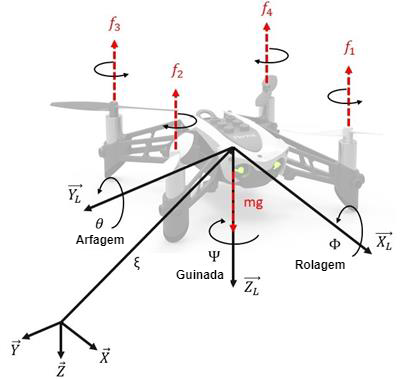
\includegraphics[width=0.6\textwidth]{coordinate-system.png}
	\caption{Representação do sistema de referência inercial e do sistema centralizado no corpo do drone. Fonte: Adaptado de Zaraza Espinosa e Buitrago Galvan (2023).}
	\centering
	\label{fig:coordinate-system}
\end{figure}


\subsection{Matrizes de rotação}
Agora que já estão estabelecidos os sistemas de referência que serão utilizados, se faz necessário relacionar o sistema de referência inercial($\boldsymbol{\vec{I}}$), que será nosso sistema de trabalho, com o sistema de referência do corpo($\boldsymbol{\vec{B}}$) obtendo assim a matriz de rotação entre os sistemas, que chamaremos de $R_{bi}$.
A matriz de rotação $R_{bi}$ é obtida através de 3 rotações sucessivas ao longo dos eixos do sistema inercial, assim a sequência utilizada nesse trabalho será a x-y-z(3-2-1), ou seja, uma rotação de ($\phi$) ao longo do eixo x (rolagem), uma rotação ($\theta$) ao longo do eixo y (arfagem) e uma rotação ($\psi$) ao longo do eixo z (guinada).
Cada rotação pode ser representada a partir de uma matriz, sendo que, a  matriz de rotação ao longo de x é:

\begin{equation*}
	R_x = \begin{pmatrix}
		1 & 0         & 0        \\
		0 & \cos\phi  & \sin\phi \\
		0 & -\sin\phi & \cos\phi
	\end{pmatrix}
\end{equation*}

A  matriz de rotação ao longo de y é:

\begin{equation*}
	R_y = \begin{pmatrix}
		\cos\theta  & 0 & \sin\theta \\
		0           & 1 & 0          \\
		-\sin\theta & 0 & \cos\theta
	\end{pmatrix}
\end{equation*}

A  matriz de rotação ao longo de z é:

\begin{equation*}
	R_z = \begin{pmatrix}
		\cos\psi  & \sin\psi & 0 \\
		-\sin\psi & \cos\psi & 0 \\
		0         & 0        & 1
	\end{pmatrix}
\end{equation*}

\includegraphics[width=1\textwidth]{matrix-rotation-explained}


Tais rotações podem ser melhor observadas na figura \ref{fig:matrix-rotation-explained}.

A matriz de transformação de referência  $R_{bi}$ que relaciona os dois sistemas de referencia, inercial e fixo ao corpo, é o produto das matrizes Rx, Ry, Rz. De forma que:


\[
	R_{bi}(\phi,\theta,\psi) = R_z(\psi) R_y(\theta) R_x(\phi) =
	\begin{bmatrix}
		cos_\theta cos_\psi & sin_\phi sin_\theta cos_\psi - cos_\phi sin_\psi & cos_\phi sin_\theta cos_\psi + sin_\phi sin_\psi \\
		cos_\theta sin_\psi & sin_\phi sin_\theta sin_\psi + cos_\phi cos_\psi & cos_\phi sin_\theta sin_\psi - sin_\phi cos_\psi \\
		-sin_\theta         & sin_\phi cos_\theta                              & cos_\phi cos_\theta
	\end{bmatrix}
\]


\section{Configurações do quadricóptero}

Como já falado o Parrot Mambo é um quadricóptero, consiste de 4 atuadores,conjunto motor e hélice, que são controlados individualmente para gerar empuxo, com o intuito de vencer a força da gravidade e atingir um voo pairado. Assim, dois dos motores tem que rodar em direções opostas, dois motores giram no sentido horáro e dois no anti-horáro, para que o momento resultante em torno do centro de massa seja zero e previna movimentos indesejados.
Além disso, o quadricóptero que vamoas analisar tem uma configuração em 'X', que têm desempenho de controle idêntico a configuração em '+', quando se trata do empuxo e do controle de guinada, mas têm aproximadamente aproximadamente 30\% de vantagem no controle quando se trata da rolagem e da arfagem, isso se dá pois o na configuração em '+', esses movimentos são feitos utilizando apenas dois motores, diferente da outra que utiliza os 4 motores(Niemiec e Gandhi, 2014). 
Os quadricópteros, independente da sua configuração, têm 6 graus de liberdade, necessários para a representação do sistema. Esses se
dividem em três para o movimento de translação nos eixos \( X \), \( Y \), \( Z \) e outros três para o movimento de rotação em cada um dos eixos \( \phi \) (rolagem), \( \theta \) (arfagem) e \( \psi \) (guinada), mas como falado o quadricóptero têm apenas 4 atuadores, então chamamos esse sistema de sub-atuado, ou seja, algumas direções não são controláveis em nenhum momento. Por exemplo, o quadricóptero não é capaz de de se mover para direita sem antes rotacionar naquela direção, o que também é válido para o movimento pra frente e pra trás, nos quais necessariamente o quadricóptero tem que realizar uma arfagem. De qualquer forma, pode-se superar essa barreira do sistema sub-atuado, seguindo o exemplo já citado, combinando rotações e empuxo para atingir o objetivo final.
Assim, para entender melhor como o quadricóptero realiza suas manobras, é importante descrever os movimentos que ele pode executar, associados aos 6 graus de liberdade. Cada movimento, está relacionado a uma combinação de empuxo gerado pelos atuadores e rotações controladas, que, como já mencionado, são executadas no intuito de superar as limitações do sistema sub-atuado.

\section{Movimentos do Quadricóptero}

\subsection{Movimento de Rolagem (Roll - $\phi$)}
A rotação em torno do eixo longitudinal ($X$) do quadricóptero, chamada de rolagem, ocorre quando os motores de um lado geram mais empuxo que os motores do lado oposto. Esse movimento inclina o quadricóptero para a direita ou esquerda, permitindo que ele se desloque lateralmente.

\begin{figure}[ht]
	\centering
	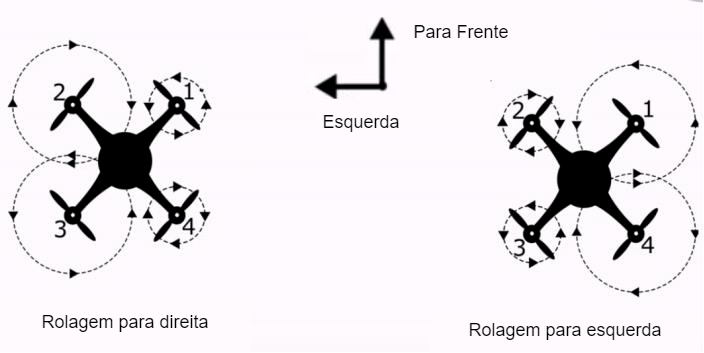
\includegraphics[width=0.8\textwidth]{rolagem-motores.png} % Substitua por seu caminho de imagem
	\caption{Modelo de Design baseado em algoritmo de rastreamento de linha para um mini drone de baixo custo por meio de controle baseado em visão (Ceppi, 2020).}
	\label{fig:line_tracking_algorithm}
\end{figure}

\begin{figure}[ht]
	\centering
	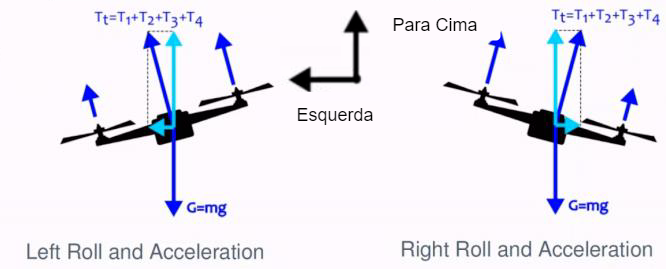
\includegraphics[width=0.8\textwidth]{rolagem-movimento.png} % Substitua por seu caminho de imagem
	\caption{Modelo de Design baseado em algoritmo de rastreamento de linha para um mini drone de baixo custo por meio de controle baseado em visão (Ceppi, 2020).}
	\label{fig:line_tracking_algorithm}
\end{figure}




\subsection{Movimento de Arfagem (Pitch - $\theta$)}
A arfagem corresponde à rotação em torno do eixo lateral ($Y$), fazendo com que o quadricóptero se incline para frente ou para trás. Esse movimento é realizado pela variação de empuxo entre os motores dianteiros e traseiros, resultando em deslocamento longitudinal (para frente ou para trás).

\begin{figure}[ht]
	\centering
	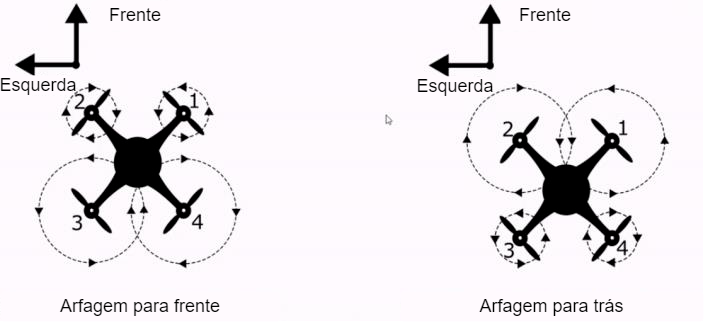
\includegraphics[width=0.8\textwidth]{arfagem-motores.png} % Substitua por seu caminho de imagem
	\caption{Modelo de Design baseado em algoritmo de rastreamento de linha para um mini drone de baixo custo por meio de controle baseado em visão (Ceppi, 2020).}
	\label{fig:line_tracking_algorithm}
\end{figure}


\begin{figure}[ht]
	\centering
	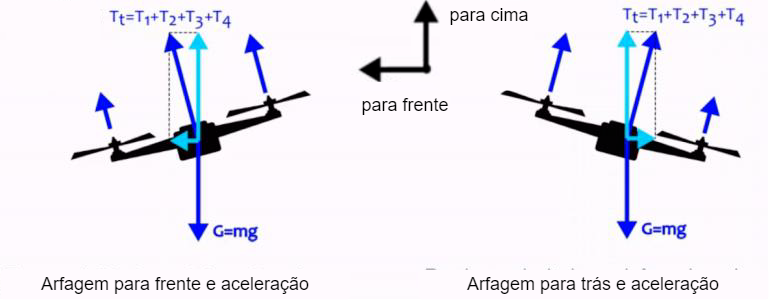
\includegraphics[width=0.8\textwidth]{arfagem-movimento.png} % Substitua por seu caminho de imagem
	\caption{Modelo de Design baseado em algoritmo de rastreamento de linha para um mini drone de baixo custo por meio de controle baseado em visão (Ceppi, 2020).}
	\label{fig:line_tracking_algorithm}
\end{figure}



\subsection{Movimento de Guinada (Yaw - $\psi$)}
A guinada refere-se à rotação em torno do eixo vertical ($Z$), que altera a direção para a qual o quadricóptero está apontando. Isso é conseguido ao variar as rotações dos motores no sentido horário e anti-horário, criando um momento resultante em torno do eixo vertical que gira o quadricóptero em sua própria base. Se todos as hélices estiverem rotacionando na mesma direção, o quadricóptero iria rotacionar em torno do eixo ($Z$) descontroladamente. Assim o quadricóptero têm 2 tipos de hélices, para que em pares elas rotacionem no sentido horário(SH) e sentido anti-horário (SAH) e cancelem o efeito da reação gerada. Logo para um movimento controlado de guinada, aumentasse o torque do par de hélices SAH, ou SH, e o quadricóptero rotaciona no sentido contrário, por conta do torque não balanceado.

\begin{figure}[ht]
	\centering
	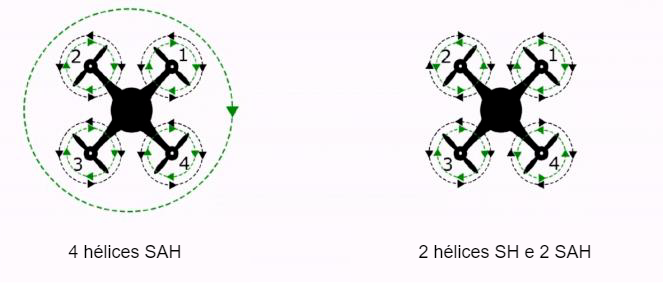
\includegraphics[width=0.8\textwidth]{guinada-motores-movimento.png} % Substitua por seu caminho de imagem
	\caption{Modelo de Design baseado em algoritmo de rastreamento de linha para um mini drone de baixo custo por meio de controle baseado em visão (Ceppi, 2020).}
	\label{fig:line_tracking_algorithm}
\end{figure}


\begin{figure}[ht]
	\centering
	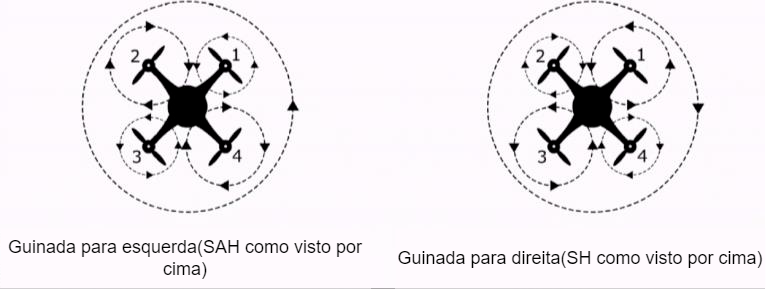
\includegraphics[width=0.8\textwidth]{guinada-movimento.png} % Substitua por seu caminho de imagem
	\caption{Modelo de Design baseado em algoritmo de rastreamento de linha para um mini drone de baixo custo por meio de controle baseado em visão (Ceppi, 2020).}
	\label{fig:line_tracking_algorithm}
\end{figure}




\subsection{Movimentos de Translação}
Os movimentos de translação são alcançados através da combinação das rotações já descritas:

\begin{itemize}
	\item \textbf{Translação no eixo X (lateral):} Consequência da inclinação em rolagem, o quadricóptero se desloca para a direita ou esquerda.
	\item \textbf{Translação no eixo Y (longitudinal):} Quando o quadricóptero realiza uma arfagem, ele se move para frente ou para trás.
	\item \textbf{Translação no eixo Z (vertical):} Controlada diretamente pela força de empuxo dos quatro atuadores, logo se o empuxo total é menor do que a força da gravidade, o quadricóptero desce e se for maior ele sobe.
\end{itemize}

Esses movimentos, coordenados pelo sistema de controle, permitem ao quadricóptero realizar voos precisos e estáveis. No entanto, como os atuadores não controlam diretamente todos os movimentos, o sistema depende da combinação inteligente de rotações e empuxos para realizar as manobras desejadas. E em resumo podemos observar que o movimento de arfagem é acoplado ao movimento de translação no eixo Y (para frente e para trás), a rolagem é acoplada ao movimento de transalação no eixo X (para esquerda e para direita) e a guinada e o momvimento de translação no eixo Z (para cima e para baixo), são graus de liberdade independentes.
Assim, é interessante e usual, que se tenha um "algoritmo de mistura dos motores", capaz de converter os comandos de rolagem, arfagem, guinada e empuxo em velocidade dos motores, o que será útil na representação do modelo no Simulink.

\begin{equation}
	\text{Motor}_{\text{frente-direita}} = \text{comando de empuxo} + \text{comando de guinada} + \text{comando de arfagem} + \text{comando de rolagem}
\end{equation}
\begin{equation}
	\text{Motor}_{\text{frente-esquerda}} = \text{comando de empuxo} - \text{comando de guinada} + \text{comando de arfagem} - \text{comando de rolagem}
\end{equation}
\begin{equation}
	\text{Motor}_{\text{trás-direita}} = \text{comando de empuxo} - \text{comando de guinada} - \text{comando de arfagem} + \text{comando de rolagem}
\end{equation}
\begin{equation}
	\text{Motor}_{\text{trás-esquerda}} = \text{comando de empuxo} + \text{comando de guinada} - \text{comando de arfagem} - \text{comando de rolagem}
\end{equation}






\subsection{Matriz de Inércia}

A massa total do quadricóptero \( m \) afeta diretamente a dinâmica translacional e a quantidade de empuxo necessário para manter o voo. Além disso, a distribuição de massa em torno do centro de gravidade é representada pela matriz de inércia \( \boldsymbol{I} \), que será utilizado nas equações de movimento rotacional.

O movimento rotacional do quadricóptero é descrito pela matriz de inércia \( \boldsymbol{I} \), que depende da distribuição de massa ao longo dos eixos principais. Para um quadricóptero simétrico como o Parrot Mambo, a matriz de inércia pode ser representado por uma matriz diagonal da forma:

\[
	\boldsymbol{I} = \begin{pmatrix}
		I_{xx} & 0      & 0      \\
		0      & I_{yy} & 0      \\
		0      & 0      & I_{zz}
	\end{pmatrix}
\]

Onde \( I_{xx} \), \( I_{yy} \) e \( I_{zz} \) são os momentos de inércia ao longo dos eixos \( X \), \( Y \) e \( Z \) do sistema de coordenadas do corpo.


Na sequência,  usaremos a matriz de rotação previamente obtida, para descrever o movimento geral do corpo a partir de suas equações de movimento translacional e rotacional.

Pode-se utilizar da matriz de rotação $R_{bi}$ para chegar na seguinte relação entre as
velocidades:


\begin{align*}
	\begin{bmatrix}
		$$ \dot{x} $$ \\
		$$ \dot{y} $$ \\
		$$ \dot{z} $$ \\
	\end{bmatrix}
	 & = R_{bi}
	\begin{bmatrix}
		u \\
		v \\
		w \\
	\end{bmatrix}
\end{align*}

Para a análise da dinâmica rotacional do movimento, iremos utilizar as equações historicamente conhecidas como equações de Euler(HIBBLER), essas equações consideram que o sistema de referência solidário ao corpo é coincidente com o centro de massa e o corpo é rígido e simétrico, fazendo que os produtos de inércia sejam zero, Ixx = Ix, Iyy = Iy, Izz = Iz:

\begin{equation}
	I \frac{d\omega}{dt} = \omega \times I \cdot \omega + H
\end{equation}

onde:

$\mathbf{I}$ é a matriz de inércia do corpo,
$\boldsymbol{\omega}$ é o vetor de velocidade angular,
$\frac{d\boldsymbol{\omega}}{dt}$ é a taxa de variação da velocidade angular,
$\times$ representa o produto vetorial,
$\boldsymbol{H}$ é o vetor do momento aplicado.

\begin{equation*}
	I = \begin{pmatrix}
		I_{xx} & 0      & 0      \\
		0      & I_{yy} & 0      \\
		0      & 0      & I_{zz}
	\end{pmatrix}
\end{equation*}

Onde Ixx, Iyy e Izz são os momentos de inércia sobre os seus eixos principais.


\subsection{Dinâmica transacional}

Usando a Segunda Lei de Newton, podemos analisar a dinâmica translacional do corpo no referencial inercial. As forças atuantes no drone sâo da tração gerada pelos 4 propulsores bem com as forças aerodinâmicas de arrasto agindo sobre o drone. Assim cada uma das forças aerodinâmicas e de tração devem ser transformadas do referencial to corpo para o referencial inercial utilizando as matrizes de transformação previamente definidas. Assim as equações de movimento translacional podem ser definidas como:


\begin{equation}
	{m}\frac{d^2}{dt^2}
	\begin{bmatrix}
		x_i \\
		y_i \\
		z_i \\
	\end{bmatrix} =
	R_{ib}\sum_{i=1}^{4}T_i -R{ib}D - m
	\begin{bmatrix}
		0 \\
		0 \\
		g
	\end{bmatrix}
\end{equation}

Sendo que na equação (1.1), Ti são os vetores de força gerado pelos motores de 1 a n, D é a força aerodinâmica de arrasto agindo no drone, m é a massa total do drone e g é aceleração da gravidade.


\subsection{Forças aerodinâmicas}

Quando falamos das forças aerodinâmicas atuando em um drone, podemos considerar que a única força externa além do arrasto é gerada pelas hélices, na forma de torque e tração. Assim geralmente assumimos que os únicos torques e trações gerados pelas hélices são utilizados para o controle do drone.


Para compreender completamente a dinâmica do movimento translacional de um drone, é crucial examinar as forças e momentos que atuam sobre o corpo. Estas podem ser decompostas em forças de propulsão, forças aerodinâmicas, arrasto e momentos devido às hélices.

1. Forças de Propulsão:

As forças de propulsão são geradas pelos motores do drone e são representadas pelos vetores $\mathbf{T}_i$. A soma vetorial dessas forças, considerada no referencial inercial ($\mathbf{F}_{\text{total}} = \sum_{i=1}^{4} \mathbf{T}_i$), constitui a força total de propulsão que impulsiona o drone.

2. Força Aerodinâmica de Arrasto (\textbf{D}):

O arrasto aerodinâmico (\textbf{D}) é a força resistiva oposta ao movimento do drone. Essa força é influenciada pela velocidade relativa do drone em relação ao ar e por características aerodinâmicas específicas do seu design.

3. Força Gravitacional $(\textbf{F}_{\text{mg}})$:

A força gravitacional $(\textbf{F}_{\text{mg}})$ atua no sentido negativo do eixo vertical e é proporcional à massa do drone ($m$) e à aceleração da gravidade ($g$).

4. Momentos devido às Hélices ($\boldsymbol{\tau}_{\phi}$, $\boldsymbol{\tau}_{\theta}$, $\boldsymbol{\tau}_{\psi}$):

Os momentos em torno dos eixos de rotação ($\phi, \theta, \psi$) são influenciados pelos torques ($\boldsymbol{\tau}_{\phi}, \boldsymbol{\tau}_{\theta}, \boldsymbol{\tau}_{\psi}$) gerados pelas hélices. Estes momentos resultam da interação entre as forças de propulsão desiguais e as distâncias entre os motores.


A equação dos torques gerados pela hélice pode ser expandida para fornecer uma visão mais detalhada dos fatores envolvidos. A equação geral para o momento ($\tau$) gerado por uma hélice é frequentemente modelada usando a equação do torque de potência. Vamos expandir essa equação:

\begin{equation}
	\tau = k_t \cdot \rho \cdot A \cdot R \cdot \Omega^2
\end{equation}

onde:

\begin{align*}
	\tau_i   & \text{ é o momento gerado pelo i-ésimo motor.}   \\
	k_t      & \text{ é o coeficiente de empuxo da hélice.}     \\
	\rho     & \text{ é a densidade do ar.}                     \\
	A        & \text{ é a área da seção transversal da hélice.} \\
	R        & \text{ é o raio efetivo da hélice.}              \\
	\Omega_i & \text{ é a velocidade angular da hélice.}
\end{align*}

Esta equação baseia-se na teoria da aerodinâmica das hélices e descreve como o torque gerado pela hélice ($\tau_i$) é proporcional ao quadrado da velocidade angular ($\Omega_i$), à densidade do ar ($\rho$), à área da seção transversal ($A$), e ao coeficiente de empuxo ($k_t$).

Além disso, é comum considerar outros fatores que afetam a eficiência do sistema de propulsão, como o efeito solo, a influência mútua entre as hélices e as perdas mecânicas. Assim, a equação do torque pode ser estendida para incorporar esses fatores:

\begin{equation}
	\tau_i = k_t \cdot \rho \cdot A \cdot R \cdot \Omega_i^2 + Q_i
\end{equation}

onde $Q_i$ representa termos adicionais que levam em conta fatores de correção e não idealidades no sistema.

A modelagem precisa dos torques é fundamental para prever o comportamento dinâmico do drone e projetar sistemas de controle eficazes. A obtenção experimental desses parâmetros é frequentemente realizada em testes de laboratório, onde a resposta das hélices a diferentes condições de operação é medida e analisada.


Os momentos aerodinâmicos referem-se aos momentos (torques) que são gerados devido às forças aerodinâmicas atuando em uma aeronave, incluindo drones. Esses momentos desempenham um papel crucial na estabilidade e controle do voo. Vamos explorar os momentos aerodinâmicos em relação aos eixos principais de um drone.

\section*{1. Momento de Rolamento $(\boldsymbol{L})$:}

O momento de rolamento (\(L\)) é gerado pela componente aerodinâmica que atua perpendicularmente ao eixo transversal da aeronave. Ele resulta em uma rotação em torno do eixo de rotação longitudinal (Roll). A relação entre o momento de rolamento aerodinâmico (\(M_{\text{aero}}\)) e a taxa de rotação angular (\(\phi\)) pode ser expressa por:

\[
	L = I_{xx} \cdot \frac{d^2 \phi}{dt^2}
\]

\section*{2. Momento de Arfagem $(\boldsymbol{M})$:}

O momento de arfagem (\(M\)) é causado pela componente aerodinâmica que atua perpendicularmente ao eixo lateral da aeronave. Ele induz uma rotação em torno do eixo de rotação transversal (Pitch). A relação com a taxa de rotação angular (\(\theta\)) é dada por:

\[
	M = I_{yy} \cdot \frac{d^2 \theta}{dt^2}
\]

\section*{3. Momento de Guinada $(\boldsymbol{N})$:}

O momento de guinada (\(N\)) é associado à componente aerodinâmica que atua perpendicularmente ao eixo vertical da aeronave. Ele resulta em uma rotação em torno do eixo vertical (Yaw). A relação com a taxa de rotação angular (\(\psi\)) é representada por:

\[
	N = I_{zz} \cdot \frac{d^2 \psi}{dt^2}
\]

Vamos estabelecer a relação entre os momentos aerodinâmicos e os torques em um drone. Isso envolve considerar como as forças aerodinâmicas aplicadas às superfícies da aeronave geram torques que influenciam sua dinâmica de rotação. Vamos analisar cada eixo separadamente:

\section*{1. Momento de Rolamento $(\boldsymbol{L})$ e Torque $(\boldsymbol{\tau_{\phi}})$:}

O momento de rolamento (\(L\)) é gerado por forças aerodinâmicas que atuam perpendicularmente ao eixo transversal da aeronave. Este momento é diretamente proporcional à taxa de rotação angular (\(\phi\)). Portanto, podemos relacionar \(L\) com o torque de rolamento (\(\tau_{\phi}\)), sendo l o tamanho do braço do motor:

\[
	L = I_{xx} \cdot \frac{d^2 \phi}{dt^2} = l \cdot \tau_{\phi}
\]

\section*{2. Momento de Arfagem $(\boldsymbol{M})$ e Torque $(\boldsymbol{\tau_{\theta}})$:}

O momento de arfagem (\(M\)) é causado por forças aerodinâmicas perpendiculares ao eixo lateral da aeronave. Ele está diretamente relacionado à taxa de rotação angular (\(\theta\)), sendo l o tamanho do braço do motor. Podemos expressar essa relação como:

\[
	M = I_{yy} \cdot \frac{d^2 \theta}{dt^2} = l \cdot \tau_{\theta}
\]

\section*{3. Momento de Guinada $(\boldsymbol{N})$ e Torque $(\boldsymbol{\tau_{\psi}})$:}

O momento de guinada (\(N\)) é associado a forças aerodinâmicas perpendiculares ao eixo vertical da aeronave e sendo l o tamanho do braço do motor. Sua relação com a taxa de rotação angular (\(\psi\)) pode ser descrita por:

\[
	N = I_{zz} \cdot \frac{d^2 \psi}{dt^2} = 0 \cdot \tau_{\phi} + 0 \cdot \tau_{\theta} + 1 \cdot \tau_{\psi}
\]


\subsection{Cinemática de Rotação}

A cinemática de rotação em drones é essencial para compreender o movimento angular sem levar em conta as forças envolvidas. Vamos explorar os fundamentos passo a passo, abordando ângulos de Euler, taxas de rotação angular.

A relação entre as velocidades angulares do corpo e as taxas de variação dos angulos de Euler, pode ser dada como:

\begin{equation}
	\omega = \Omega \dot{\Theta}
\end{equation}

As taxas de rotação angular ($\dot{\phi}$, $\dot{\theta}$, $\dot{\psi}$) são as derivadas dos ângulos de Euler. Utilizamos a matriz de rotação das velocidades angulares para relacionar as velocidades angulares às taxas de rotação(p,q,r) ao redor dos eixos x, y, e z:

\[
	\begin{bmatrix}
		\dot{\phi}   \\
		\dot{\theta} \\
		\dot{\psi}
	\end{bmatrix}
	=
	\begin{bmatrix}
		1 & \sin(\phi) \cdot \tan(\theta) & \cos(\phi) \cdot \tan(\theta) \\
		0 & \cos(\phi)                    & -\sin(\phi)                   \\
		0 & \sin(\phi)/\cos(\theta)       & \cos(\phi)/\cos(\theta)
	\end{bmatrix}
	\begin{bmatrix}
		p \\
		q \\
		r
	\end{bmatrix}
\]

Essa relação nos permite converter as taxas de rotação angular para as taxas de variação dos ângulos de Euler.

Aqui, podemos aplicar a suposição para pequenos ângulos, assumindo que o sistema nâo alcançará angulos elevados, sendo que isso invalidaria a modelagem. Logo, podemos fazer as seguintes aproximações, \[ \cos(\delta) =1\] , \[ \sin(\delta) =\delta\], o que nos dá:
\[ p = \dot{\phi} - \theta\dot{\psi} \]

\[ q = \dot{\theta} + \phi\dot{\psi}\]

\[ r = - \psi\dot{\theta} + \dot{\psi} \]

Assim, considerando pequenas velocidades angulares, o termos com multiplicação podem ser considerados pequenos o suficiente para serem eliminados, de forma que ficamos com:
\[
	\begin{bmatrix}
		\omega_{x} \\
		\omega_{y} \\
		\omega_{z}
	\end{bmatrix}
	=
	\begin{bmatrix}
		p \\
		q \\
		r
	\end{bmatrix}
	=
	\begin{bmatrix}
		\dot{\phi}   \\
		\dot{\theta} \\
		\dot{\psi}
	\end{bmatrix}
\]

Derivando em função do tempo, temos:
\[
	\begin{bmatrix}
		\dot{\omega_{x}} \\
		\dot{\omega_{y}} \\
		\dot{\omega_{z}}
	\end{bmatrix}
	=
	\begin{bmatrix}
		\ddot{\phi}   \\
		\ddot{\theta} \\
		\ddot{\psi}
	\end{bmatrix}
\]



\subsection{Dinâmica de Rotação}

A dinâmica de rotação em drones explora como os torques aplicados a uma aeronave influenciam suas taxas de rotação angular. Vamos passar por todos os passos do equacionamento, começando pela Segunda Lei de Newton para a rotação.

\[ \vec{M} = \dot{\vec{H}} \ \ \ (2.9) \]


Sendo que \(\vec{M}\) representa a soma total de todos os momentos que afetam a rotação do drone. Inclui contribuições externas, como os gerados pelos motores e forças aerodinâmicas, e contribuições internas, como os momentos inerciais resultantes da distribuição de massa.
O termo, \(\vec{H}\) denota a variação do momento angular. O momento angular total de um quadrirotor compreende duas componentes distintas. A primeira delas diz respeito à rotação do próprio corpo, enquanto a segunda está relacionada à rotação dos motores. Portanto,

\[ \vec{H} = \vec{H}_{\text{corpo}} + \vec{H}_{\text{motores}} \ \ \ (2.10) \]

Onde \(\vec{H}_{\text{corpo}}\) representa o momento angular do corpo e \(\vec{H}_{\text{motores}}\) corresponde ao momento angular devido aos motores. Esses momentos angulares podem ser descritos da seguinte forma:

\[ \vec{H}_{\text{corpo}} = \vec{I}_{\text{corpo}} \cdot \vec{\omega}_{\text{corpo}} \ \ \ (2.11) \]

\[ \vec{H}_{\text{motores}} = \begin{bmatrix} 0 \\ 0 \\ J_r \Omega \end{bmatrix} \ \ \ (2.12) \]

Aqui, \(J_r\) representa o momento de inércia do conjunto composto pelo rotor, eixo e hélice, enquanto \(\Omega\) é a velocidade nominal de rotação do motor. Portanto, a equação de Euler que descreve a dinâmica de rotação é definida como:

\[ \dot{\vec{I}_{\text{corpo}} \cdot \vec{\omega}_{\text{corpo}}} = \vec{M} - \vec{\omega}_{\text{corpo}} \times (\vec{H}_{\text{corpo}} + \vec{H}_{\text{motores}}) \ \ \ (2.13) \]

Para cada um dos eixos, temos:

% Roll (eixo x)
\[
	I_{xx} \cdot \dot{\phi} = (I_{zz} - I_{yy}) \cdot \dot{\theta} \cdot \dot{\psi} + H_{\phi}
\]

% Pitch (eixo y)
\[
	I_{yy} \cdot \dot{\theta} = (I_{xx} - I_{zz}) \cdot \dot{\phi} \cdot \dot{\psi} + H_{\theta}
\]

% Yaw (eixo z)
\[
	I_{zz} \cdot \dot{\psi} = (I_{yy} - I_{xx}) \cdot \dot{\phi} \cdot \dot{\theta} + H_{\psi}
\]

Os termos \(\dot{\vec{I}_{\text{corpo}}  \vec{\omega}_{\text{corpo}}}\)    e    \(\vec{\omega}_{\text{corpo}} \times (\vec{H}_{\text{corpo}} + \vec{H}_{\text{motores}})\) representam a taxa de variação do momento angular no sistema do corpo. O operador de produto vetorial \(\times\) é aplicado na última parte da equação.

Isolando os momentos H e os relacionando com os momentos aerodinâmicos, temos:

% Roll (eixo x)
\[
	I_{xx} \cdot \frac{d\omega_{\phi}}{dt} + (I_{yy} - I_{zz}) \cdot \omega_{\theta} \cdot \omega_{\psi} = I_{xx} \cdot \frac{d^2\phi}{dt^2}
\]

% Pitch (eixo y)
\[
	I_{yy} \cdot \frac{d\omega_{\theta}}{dt} + (I_{zz} - I_{xx}) \cdot \omega_{\phi} \cdot \omega_{\psi} = I_{yy} \cdot \frac{d^2\theta}{dt^2}
\]

% Yaw (eixo z)
\[
	I_{zz} \cdot \frac{d\omega_{\psi}}{dt} + (I_{xx} - I_{yy}) \cdot \omega_{\phi} \cdot \omega_{\theta} = I_{zz} \cdot \frac{d^2\psi}{dt^2}
\]
\ \ \ (2.15)

\subsection{Modelo dinâmico do quadricóptero}

Assim, considerando (1.2) e (2.15), e as considerações feitas ao longo deste capítulo, podemos chegar ao modelo dinâmico do quadricóptero dado por:

\begin{align*}
	\ddot{x}     & = -(\cos\phi \cos\psi \sin\theta + \sin\phi \sin\psi)T_m                            \\
	\ddot{y}     & = -(\cos\phi \sin\psi \sin\theta - \sin\phi \cos\psi)T_m                            \\
	\ddot{z}     & = g - \cos\phi \cos\theta T_m                                                       \\
	\dot{\phi}   & = -\dot{\theta}\dot{\psi}(I_{zz} - I_{yy}) - \dot{\theta}J_r\Omega_{Ixx} + L I_{xx} \\
	\dot{\theta} & = -\dot{\phi}\dot{\psi}(I_{xx} - I_{zz}) + \dot{\phi}J_r\Omega_{Iyy} + M I_{yy}     \\
	\dot{\psi}   & = -\dot{\phi}\dot{\theta}\frac{I_{yy} - I_{xx}}{I_{zz}} + N I_{zz}
\end{align*}




%---------------------------------------------------------------------
% INDICE REMISSIVO
%---------------------------------------------------------------------
\phantompart
\printindex
%---------------------------------------------------------------------
